\documentclass[11pt,oneside]{book}

\usepackage[french]{babel}
\usepackage[utf8]{inputenc}  
\usepackage[T1]{fontenc}
\usepackage{listings}
\usepackage{comment}
\usepackage[left=2.5cm,right=2.5cm,top=3cm,bottom=2.65cm]{geometry}
\usepackage{graphicx}
\usepackage{tabularx}
\usepackage{amsmath,amssymb,amsfonts}
\usepackage{bbm, bm}
\usepackage{stmaryrd}
\usepackage{mathtools}
\usepackage{hyperref}
\usepackage{tikz}
\usepackage{tabularx}
\usepackage{makecell}
\usepackage{color}
\usepackage{fancybox}
\usepackage[thmmarks,amsmath]{ntheorem}
\usepackage{minitoc}
\usepackage{titletoc}
\usepackage{tikz}
\usepackage{algpseudocode}
\usepackage[]{algorithm2e}
\usepackage{wrapfig}
\usepackage{kpfonts}

\graphicspath{{images/}}

\DeclareMathOperator*{\argmax}{arg\,max}
\DeclareMathOperator*{\argmin}{arg\,min}

\usetikzlibrary{arrows.meta}
\usetikzlibrary{arrows}
\mathtoolsset{showonlyrefs=true}

\addto\extrasfrench{%
	\def\subsectionautorefname{\S}%
	\def\sectionautorefname{\S}%
}

\definecolor{darkWhite}{rgb}{0.94,0.94,0.94}
\definecolor{blue}{rgb}{0.12,0.16,0.53}
\definecolor{green}{rgb}{0.25,0.28,0.06}
\definecolor{greenTikz}{rgb}{0.16,0.53,0.12}
\definecolor{red}{rgb}{0.71,0.19,0.11}
\definecolor{darkPurple}{rgb}{0.2,0.05,0.18}
\definecolor{whiteGray}{rgb}{0.92,0.96,0.95}

\newcounter{sss}
\renewcommand\thesection{\textcolor{red}{\Roman{section} -}}
\renewcommand\thesubsection{\textcolor{blue}{\arabic{subsection}/}}
\renewcommand\thesss{\textcolor{green}{\alph{sss}.}}
\renewcommand\thechapter{\Alph{chapter}}
\newcommand{\sect}[1]{\section{\textcolor{red}{#1}}}
\newcommand{\subs}[1]{\subsection{\textcolor{blue}{#1}}}
\newcommand{\subsubs}[1]{
	\stepcounter{sss}
	\subsubsection{\textcolor{green}{\thesss~#1}}
}

\newcommand{\mybox}[4]{
	\begin{center}
		\boxput*(0,1){\colorbox{darkWhite}{\textbf{#1}}}{
			\setlength{\fboxsep}{12pt}
			\fcolorbox{#2}{#3}{
				\begin{Bflushleft}
					\begin{minipage}{0.908\linewidth}
						\vspace{2mm} \par \textcolor{#2}{#4}
					\end{minipage}
				\end{Bflushleft}
			}
		}
	\end{center}
}

\newcommand{\mytitle}[1]{
	\title{
		\fcolorbox{black}{whiteGray}{
			\begin{Bflushleft}
				\\ \huge \textbf{\textcolor{red}{#1}}
			\end{Bflushleft}
		}
	}
}

\setcounter{tocdepth}{1}
\setcounter{minitocdepth}{3}
\nomtcrule
\titlecontents*{chapter}[0pt]{}
{\bfseries\chaptername\ \thecontentslabel\quad}{}
{\bfseries\hfill\contentspage}
\newcommand{\mytoc}{
	\renewcommand{\contentsname}{}
	\mybox{Table des matières}{darkPurple}{darkWhite}{
		\vspace{-40mm}\tableofcontents}
}
\newcommand{\myminitoc}{
	\mybox{Table des matières}{darkPurple}{darkWhite}{
		\vspace{-9mm}\minitoc \vspace{-8mm}}
}


\newcommand{\DEF}[1]{\vspace{1mm} \mybox{Définition}{blue}{white}{#1}}
\newcommand{\REM}[1]{\vspace{1mm} \mybox{Remarque}{darkPurple}{white}{#1}}

\newcounter{propNum}
\newcommand{\PROP}[2][]{
	\stepcounter{propNum}
	\vspace{1mm}
	\mybox{Proposition \thepropNum #1}{red}{white}{#2}
}
\newcommand{\dem}{\paragraph{Démonstration}}
\newcommand{\findem}{\hfill $\blacksquare$}
\newcommand{\exe}{\paragraph{\textit{\textcolor{green}{Exemple}}}}

\newcommand{\N}{\mathbb{N}}
\newcommand{\trans}{\mathsf{T}}
\newcommand{\R}{\mathbb{R}}
\newcommand{\Pp}{\mathbb{P}}
\newcommand{\E}{\mathbb{E}}
\newcommand{\X}{\mathcal{X}}
\newcommand{\Y}{\mathcal{Y}}
\newcommand{\Z}{\mathcal{Z}}
\newcommand{\dist}{\mathcal{D_Z}}
\newcommand{\Hyp}{\mathcal{H}}
\newcommand{\trisk}{\mathcal{R}^l}
\newcommand{\erisk}{\hat{\mathcal{R}}^l}
\newcommand{\vrisk}{\tilde{\mathcal{R}}}

\mytitle{Machine Learning}
\author{
	Notes écrites par \\
	Yoann Coudert--Osmont \\
	\texttt{yoann.coudert-osmont@ens-lyon.fr}
	\and
	D'après un cours de \\
	Marc Sebban \\
	University of Jean Monnet Saint-Étienne
}
\date\today

\begin{document}
	
	\dominitoc[n]
	\maketitle
	\mytoc
	
	\chapter{Introduction, apprentissage supervisé, bornes}

\myminitoc

\sect{Introduction}

\paragraph{Qu'est ce que le machine learning ?}
Le machine learning est le développement d'algorithmes qui apprennent tout seul à partir de données. On distingue deux catégorie :
\begin{itemize}
	\item L'apprentissage supervisé : qui apprend avec des données étiquetées afin de faire de la classification, de la régression ou encore de la hiérarchisation.
	\item  L'apprentissage non supervisé : qui trouve la structure d'un jeu de données afin de faire du clustering ou de la réduction de dimensions.
\end{itemize}
Les applications principales du machine learning sont alors la vision par ordinateur, la robotique, la reconnaissance vocale, le traitement du langage, etc ...

\sect{Apprentissage supervisé}

\DEF{
	Dans la suite on utilisera les notations suivantes :
	\begin{itemize}
		\item On pose $\bm{S = \{ z_i = (x_i, y_i) \}_{i = 1}^m}$ un ensemble de $\bm{m}$ exemples d'entraînement indépendants et identiquement distribués selon une une distribution inconnue $\bm{\dist}$ sur l'espace $\bm{\Z = \X \times \Y}$.
		\item Les valeurs $x_i \in \bm{\X}$ sont généralement des vecteurs de $\R^d$ dont les composantes sont appelées les \textbf{features}.
		\item Les valeurs $y_i \in \bm{\Y}$ se trouvent dans l'ensemble discret des \textbf{classes/étiquettes} (typiquement $\Y = \{ -1, +1 \}$ en classification binaire) ou dans un ensemble continue dans le cas de régressions.
		\item Finalement on cherche une \textbf{fonction cible} $\bm{f}$ tel que $\bm{\forall (x, y) \in \X \times \Y, \, y = f(x)}$.
	\end{itemize}
}

\DEF{
	Un \textbf{algorithme d'apprentissage supervisé} $\bm{L}$ prend en entrée $S$ et retourne un modèle ou une classification $\bm{h \in \Hyp}$ le plus proche possible de $f$.
}

\exe
Si on prend pour $f$ la fonction qui retourne {\color{red}$y = +1$} si $x_1^2 + x_2^2 < R^2$ et {\color{blue}$y = -1$} sinon, alors voici le résultat que l'on peut obtenir :
\begin{center}
	\begin{tikzpicture}[thick, scale=1.2]
		\draw[greenTikz, opacity=0.4] (0, 0) circle (1);
		\node[greenTikz] at (0.8, -0.9) {$f$};
		\draw[blue] (-2, 0) -- (2, 0) node[below left, black] {$x_1$};
		\draw[blue] (0, -2) -- (0, 1.8) node[above, black] {$x_2$};
		\draw[fill, red] (0.2, 0.7) circle (0.08);
		\draw[fill, red] (-0.4, -0.5) circle (0.08);
		\draw[fill, red] (0.2, -0.3) circle (0.08);
		\draw[fill, red] (-0.3, 0.3) circle (0.08);
		\draw[fill, red] (0.4, 0.2) circle (0.08);
		\draw[orange, very thick] (0.2, -1.5)
			.. controls (-0.5, -1) and (-1, -0.2) .. (-0.95, -0.05)
			.. controls (-1, 0.2) and (-0.4, 1) .. (0.3, 0.9)
			.. controls (0.9, 0.75) and (1, 0) .. (1.1, -0.4)
			.. controls (1.15, -0.6) and (1.05, -1.2) .. (0.8, -1.5) node[below] {$h$};
		\draw[fill, blue] (-1.1, 0.3) circle (0.08);
		\draw[fill, blue] (-1.2, -0.1) circle (0.08);
		\draw[fill, blue] (-1.3, -0.5) circle (0.08);
		\draw[fill, blue] (-1.2, -0.8) circle (0.08);
		\draw[fill, blue] (-0.8, -1.2) circle (0.08);
		\draw[fill, blue] (-0.3, -1.5) circle (0.08);
		\draw[fill, blue] (-0.6, 1) circle (0.08);
		\draw[fill, blue] (-0.9, 0.8) circle (0.08);
		\draw[fill, blue] (-0.95, 1.2) circle (0.08);
		\draw[fill, blue] (-0.2, 1.3) circle (0.08);
		\draw[fill, blue] (0.3, 1.1) circle (0.08);
		\draw[fill, blue] (0.7, 0.9) circle (0.08);
		\draw[fill, blue] (1.1, 0.5) circle (0.08);
		\draw[fill, blue] (1.3, 0.1) circle (0.08);
		\draw[fill, blue] (1.3, -0.4) circle (0.08);
		\draw[fill, blue] (1.25, -1.2) circle (0.08);
	\end{tikzpicture}
\end{center}
Ici $h$ convient aux données d'entraînement mais n'est toujours pas bon pour la généralisation.

\paragraph{Conjecture}
Plus l'ensemble $S$ sera grand, plus la fonction $h$ sera proche de $f$.

\paragraph{Malédiction de la dimensionnalité}
Quand le nombre de features augmente, le nombre $m$ d'exemples d'entraînement nécessaires pour généralisé de manière assez précise augmente exponentiellement.

\DEF{
	En statistiques, l'\textbf{overfitting} est le phénomène où le modèle obtenu est trop complexe. Il peu avoir trop de degrés de liberté par exemple. En revanche l'\textbf{underfitting} est lorsque le modèle n'arrive pas à trouver la tendance des données. 
}

\subs{Risque et fonction de perte}

\DEF{
	En théorie, on aime considéré la meilleurs hypothèse $h^* \in \Hyp$. En se donnant une \textbf{fonction de perte} $l : \Hyp \times \Z \rightarrow \R$ mesurant le degré d'accord entre $h(x)$ et $y$, le \textbf{vrai risque} ou \textbf{erreur de généralisation} $\trisk(h)$ est défini ainsi :
	$$ \trisk(h) = \E_{z \sim \dist} l(h, z) = \int_z f_\dist(z) l(h, z)$$
	$$ h^* = \argmin_{h \in \Hyp} \trisk(h) $$
	\vspace{-5mm}
}

Malheureusement, $\trisk(h)$ ne peut pas être calculé car $\dist$ est inconnu. On peut seulement calculé le \textbf{risque empirique} sur $S$. C'est à dire :
$$ \erisk(h) = \E_{z \sim S} l(h, z) = \frac{1}{m} \sum_{i = 1}^{m} l(h, z_i) $$
Ainsi le but de l'algorithme d'apprentissage supervisé est de trouver le modèle $\displaystyle h = \argmin_{h_i \in \Hyp} \erisk(h_i)$.

\exe
La fonction de perte la plus naturelle pour la classification binaire est le 0/1 loss.
$$ l_{0/1}(h, z) = \left\{ \begin{array}{ll}
	1 & \text{si } yh(x) < 0 \\
	0 & \text{sinon}
\end{array}
\right. $$
Ainsi $\mathcal{R}^{l_{0/1}}(h)$ est la proportion de mauvaises prédictions. \\
Malheureusement, à cause de la non-convexité et de la non-différentiabilité de cette fonction de perte, minimiser, ou même minimiser approximativement $\mathcal{\hat{R}}^{l_{0/1}}(h)$ est un problème NP-difficile.

\paragraph{Fonctions de perte usuelles} Pour cette raison, on utilise généralement les fonctions de perte convexes suivante :
\begin{itemize}
	\item La \textbf{perte exponentielle} (utilisée en boosting) : $l_{exp}(h, z) = e^{-yh(x)}$
	\item La \textbf{perte logistique} (utilisée en régression logistique) : $l_{log}(h, z) = \ln(1 + e^{-yh(x)})$
	\item La \textbf{perte charnière} (utilisée en SVM) : $l_{hinge}(h, z) = \max(0, 1 - yh(x))$
\end{itemize}
\begin{center}
	\begin{tikzpicture}[yscale=1.25, xscale=1.65, thick]
		\draw (-2, -0.5) node[below] {-2} -- (2, -0.5) node[below] {2};
		\draw (-2, -0.5) node[left] {-0.5} -- (-2, 3.5) node[left] {3.5};
		\draw (0, -0.5) node[] {\tiny |} node[below] {0};
		\draw (-2, 1.5) node[] {\tiny -} node[left] {1.5};
		\draw (-2, 1) node[left] {1} -- (0, 1) -- (0, 0) -- (2, 0);
		\draw[red] (-2, 3) -- (1, 0) -- (2, 0);
		\draw[domain=-1.25:2, smooth, variable=\x, blue] plot ({\x}, {exp(-\x)});
		\draw[domain=-2:2, smooth, variable=\x, greenTikz] plot ({\x}, {ln(1 + exp(-\x))});
		\draw (1.8, 3.3) -- (1.3, 3.3) node[left] {\footnotesize 0/1 loss};
		\draw[red] (1.8, 3) -- (1.3, 3) node[left] {\footnotesize hinge loss};
		\draw[greenTikz] (1.8, 2.7) -- (1.3, 2.7) node[left] {\footnotesize logistic loss};
		\draw[blue] (1.8, 2.4) -- (1.3, 2.4) node[left] {\footnotesize exponential loss};
	\end{tikzpicture}
\end{center}

\subs{Minimisation de risque régularisée}

Trop entraîner l'algorithme sur les données d'entraînement $S$ peut conduire à une mémorisation et à l'overfitting. Le modèle devient compliqué et on risque d'avoir une mauvaise généralisation. \\
Le principe du \textbf{rasoir d'Occam} est "le plus simple est le mieux". Pour appliquer ce principe, on essaye de minimiser les paramètres du modèle. \\
On va donc minimiser le \textbf{risque empirique régularisé} :
$$ \min_{h \in \Hyp} \erisk(h) + \lambda \| h \| $$
On pénalise alors les hypothèses avec une forte norme.

\DEF{
	La norme $l_p$ d'un vecteur $\theta$ d'un espace à $d$ dimensions est défini comme suit :
	$$ \| \theta \|_p = \left( \sum_{i = 1}^d |\theta_i|^p \right)^{\frac{1}{p}} $$
	\vspace{-5mm}
}

\begin{center}
	\begin{tikzpicture}[thick, >={latex}, scale=0.8]
		\draw[->] (0, 0) -- (2, 0);
		\draw[->] (1, -1) node[below] {$p=0$} -- (1, 1);
		\draw[red, very thick] (0.3, 0) -- (1.7, 0);
		\draw[red, very thick] (1, -0.7) -- (1, 0.7);
		
		\draw[->] (3, 0) -- (5, 0);
		\draw[->] (4, -1) node[below] {$p=0.3$} -- (4, 1);
		\draw[domain=-1:1, smooth, variable=\x, red, very thick]
			plot ({0.8*\x+4}, {0.8 * max(0.01, 1 - abs(\x)^0.3)^(1/0.3)});
			\draw[domain=-1:1, smooth, variable=\x, red, very thick]
			plot ({0.8*\x+4}, {-0.8 * max(0.01, 1 - abs(\x)^0.3)^(1/0.3)});
			
		\draw[->] (6, 0) -- (8, 0);
		\draw[->] (7, -1) node[below] {$p=0.5$} -- (7, 1);
		\draw[domain=-1:1, smooth, variable=\x, red, very thick]
			plot ({0.8*\x+7}, {0.8 * max(0.01, 1 - abs(\x)^0.5)^(1/0.5)});
		\draw[domain=-1:1, smooth, variable=\x, red, very thick]
			plot ({0.8*\x+7}, {-0.8 * max(0.01, 1 - abs(\x)^0.5)^(1/0.5)});
		
		\draw[->] (9, 0) -- (11, 0);
		\draw[->] (10, -1) node[below] {$p=1$} -- (10, 1);
		\draw[red, very thick] (9.2, 0) -- (10, 0.8) -- (10.8, 0) -- (10, -0.8) -- (9.2, 0);
		
		\draw[->] (12, 0) -- (14, 0);
		\draw[->] (13, -1) node[below] {$p=1.5$} -- (13, 1);
		\draw[domain=-1:1, smooth, variable=\x, red, very thick]
			plot ({0.8*\x+13}, {0.8 * max(0.01, 1 - abs(\x)^1.5)^(1/1.5)});
		\draw[domain=-1:1, smooth, variable=\x, red, very thick]
			plot ({0.8*\x+13}, {-0.8 * max(0.01, 1 - abs(\x)^1.5)^(1/1.5)});
		
		\draw[->] (15, 0) -- (17, 0);
		\draw[->] (16, -1) node[below] {$p=2$} -- (16, 1);
		\draw[red, very thick] (16, 0) circle (0.8);
		
		\draw[->] (18, 0) -- (20, 0);
		\draw[->] (19, -1) node[below] {$p=inf$} -- (19, 1);
		\draw[red, very thick] (18.2, 0.8) -- (19.8, 0.8) -- (19.8, -0.8) -- (18.2, -0.8) -- (18.2, 0.8);
	\end{tikzpicture}
\end{center}

La norme $l_2$ est utilisée pour réduire les risques d'overfitting en réduisant les plus grandes valeurs du modèle. La norme $l_1$, elle permet d'obtenir des modèles sparses, c'est à dire avec peu de features.

\exe
Considérons le problème suivant :
$$ \min_{\theta \in \R^d} \frac{1}{2} \theta^\trans \theta - \theta^\trans x + \lambda \| \theta \|_2^2 $$
Si $\lambda = 0$, alors :
$$ \dfrac{\partial \frac{1}{2} \theta^\trans \theta - \theta^\trans x}{\partial \theta_j} = 0 \Rightarrow \theta_j - x_j = 0 \Rightarrow \fbox{$\theta_j = x_j$} $$
Si $\lambda \neq 0$, alors :
$$ \dfrac{\partial \frac{1}{2} \theta^\trans \theta - \theta^\trans x  + \lambda \| \theta \|_2^2}{\partial \theta_j} = 0 \Rightarrow \theta_j - x_j +2\lambda \theta_j = 0 \Rightarrow \fbox{$\theta_j = \dfrac{x_j}{1 + 2\lambda}$} $$
\begin{center}
	\begin{tikzpicture}[>={latex}, thick]
	\draw[->] (-1, 0) -- (5, 0);
	\draw[->] (0, -1) -- (0, 3.5);
	\draw (3, 0) node {\tiny |} node[below] {3};
	\draw (0, 2) node {\tiny -} node[left] {2};
	\draw[fill] (3, 2) circle (0.05) node[below] {$x$};
	\draw[fill=greenTikz, fill opacity=0.5, very thick] (3, 2) circle (1.4^0.5);
	\draw[very thick] (3, 2) circle (1) circle (0.6^0.5) circle (0.2^0.5);
	\node[color=red] at (1, -0.6) {$\lambda = 0$};
	
	\draw[->] (7, 0) -- (13, 0);
	\draw[->] (8, -1) -- (8, 3.5);
	\draw (11, 0) node {\tiny |} node[below] {3};
	\draw (8, 2) node {\tiny -} node[left] {2};
	\draw[fill] (11, 2) circle (0.05) node[below] {$x$};
	\draw[fill=greenTikz, fill opacity=0.5, very thick] (9, 0.67) circle (0.47^0.5);
	\draw[very thick] (9, 0.67) circle (0.33^0.5) circle (0.2^0.5) circle (0.07^0.5);
	\node[color=red] at (9, -0.6) {$\lambda = 1$};
	\end{tikzpicture}
\end{center}

\exe
Maintenant on peut prendre la norme $l_1$ pour constater qu'elle engendre bien de la sparsité.
$$ \min_{\theta \in \R^d} \frac{1}{2} \theta^\trans \theta - \theta^\trans x + \lambda \| \theta \|_1 $$
Si $\lambda = 0$, on a vu que $\theta^* = x$. \\
En revanche si $\lambda > 0$, on considère la dérivée partielle à $\theta_j = 0^+$, et à $\theta_j = 0^-$ :
$$ g_+^j = \lambda - x_j \qquad g_-^j = - \lambda - x_j $$
Or $\theta_j^* = 0$ si et seulement si $g_+^j \geqslant 0$ et $g_-^j \leqslant 0$. C'est à dire si $x_j \geqslant \lambda$ et $x_j \leqslant -\lambda$. \\
Donc si $|x_j| \leqslant \lambda$ alors $\theta_j^* = 0$.
\begin{center}
	\begin{tikzpicture}[>={latex}, thick, scale=0.8]
	\draw[->] (-1, 0) -- (5, 0);
	\draw[->] (0, -1) -- (0, 3.5);
	\draw (3, 0) node {\tiny |} node[below] {3};
	\draw (0, 2) node {\tiny -} node[left] {2};
	\node[color=red] at (1, -0.6) {$\lambda = 0$};
	\draw[fill] (3, 2) circle (0.05) node[below] {$x$};
	\draw[fill=greenTikz, fill opacity=0.5, very thick] (3, 2) circle (5^0.5);
	\draw[very thick] (3, 2) circle (3^0.5) circle (1);
	
	\draw[->] (7, 0) -- (13, 0);
	\draw[->] (8, -1) -- (8, 3.5);
	\draw (11, 0) node {\tiny |} node[below] {3};
	\draw (8, 2) node {\tiny -} node[left] {2};
	\draw[fill] (11, 2) circle (0.05) node[below] {$x$};
	\draw[fill, red] (9, 0) circle (0.05) node[above] {$\theta^*$};
	\node[color=red] at (12.4, 3) {$\lambda = 2$};
	\node[color=red] at (12.4, 2.5) {$\theta^*$ est sparse};
	\draw[very thick, fill=greenTikz, fill opacity=0.5] (11.24, 0) arc (0:116.6:2.24);
	\draw[very thick, fill=greenTikz, fill opacity=0.5] (8, 2) arc (158:180:5.39);
	\draw[very thick, fill=greenTikz, fill opacity=0.5] (7.61, 0) arc (217:222.4:6.71);
	\draw[very thick, fill=greenTikz, fill opacity=0.5] (8, -0.47) arc (257.4:299.1:4.58);
	\draw[very thick] (10, 0) arc(0:180:1);
	\draw[very thick] (8, 0) arc(-104:-76:4.12);
	\draw[very thick] (10.73, 0) arc(0:125:3^0.5);
	\draw[very thick] (7.8, 0) arc(180:164:27^0.5);
	\draw[very thick] (7.8, 0) arc(217.6:220.5:43^0.5);
	\draw[very thick] (10.73, 0) arc(-66.6:-103:19^0.5);
	\fill[greenTikz, opacity=0.5] (11.24, 0) -- (8, 2) -- (7.61, 0) -- (8, -0.47);
	\end{tikzpicture}
\end{center}

\paragraph{Supprimer des groupes de features}
Voici des normes qui permettent de supprimer les features en groupe :
\begin{center}
	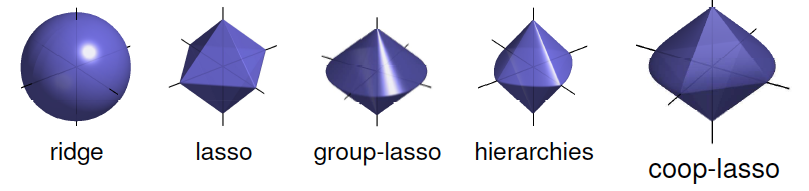
\includegraphics[scale=0.5]{group_sparse.png}
\end{center}
On considère $\{ \mathcal{G}_{k = 1}^K \}$ une partition de $\{ 1, \dots, d \}$. On peur alors définir les normes suivantes :
$$ \| \theta \|_{group} = \sum_{g \in \mathcal{G}} \left( \sum_{j \in g} \theta_j^2 \right)^{\frac{1}{2}} $$
$$ \| \theta \|_{coop} = \sum_{g \in \mathcal{G}} \left[ \left( \sum_{j \in g} [\theta_j]_+^2 \right)^{\frac{1}{2}} + \left( \sum_{j \in g} [\theta_j]_-^2 \right)^{\frac{1}{2}} \right] $$


\subs{Contrepartie Biais/Variance}

D'où vient l'erreur de $h \in \Hyp$ ?
\begin{itemize}
	\item Du \textbf{biais inductif}. Rien ne garantie l'égalité entre l'espace cible des concepts $\mathcal{F}$ et la classe d'hypothèse que l'on a choisi $\Hyp$.
	\item De la \textbf{variance}. Comme l'ensemble d'entraînement est fini et choisi aléatoirement selon $\dist$, l'algorithme d'apprentissage ne retourne pas l'hypothèse optimale $h^*$ de $\Hyp$.
\end{itemize}

\begin{center}
	\begin{tikzpicture}[thick]
		\draw (0, 0.5) -- (4, 0.5) -- (4, 2) -- node[above] {$\Hyp$} (0, 2) -- (0, 0.5);
		\node at (5.5, 0.5) {$\mathcal{F}$};
		\draw[fill] (0.5, 1) circle (0.05) node[above] {$h$}
			-- node[below, sloped] {\footnotesize erreur totale} (3.7, -1)
				circle (0.05) node[right] {$f$}
			-- node[above, sloped] {\footnotesize biais} (2.5, 1)
				circle (0.05) node[above] {$h^*$}
			-- node[above] {\footnotesize Variance} (0.5, 1);
	\end{tikzpicture}
\end{center}
$$ \trisk(h) \leqslant \text{Biais} + \text{Variance} $$
$$ \trisk(h) \leqslant \text{Biais inévitable} + \text{Biais évitable} + \text{Variance} $$
$$ \trisk(h) \leqslant {\color{red}\text{Erreur de Bayes}} + {\color{blue}\text{Biais évitable}} + {\color{blue}\text{Variance}} $$

\DEF{
	L'\textbf{erreur de Bayes} $\epsilon_B$ est le plus petit taux d'erreur pour une hypothèse $h$ :
	$$ \epsilon_B = \sum_i \int_{(x, y) \in R_i \times \bar{C_i}} P(C_i | x) p(x) dx $$
	Où $x$ est une instance avec $y$ pour étiquette et $R_i$ est la région que la fonction de classification $h$ classifie comme $C_i$.
}
\begin{center}
	C'est un $\ll$ sept $\gg$ ou un $\ll$ un $\gg$ ? \\
	
\includegraphics[scale=0.4]{one_seven.png}
\end{center}

\paragraph{Variance}
$h$ va converger vers $h^*$ si on augmente le nombre d'exemples $m$.
\begin{center}
	\begin{tikzpicture}[thick, scale=0.9]
		\draw[ultra thick, blue, opacity=0.8] (0, -2.5) -- (0, 2.5);
		\draw[ultra thick, blue, opacity=0.8] (-1.6, -2.5) -- (0.25, 2.5);
		\node[below] at (-1.6, -2.5) {$h$};
		\node[below] at (0, -2.5) {$h^*$};
		\draw[<->, red] (-0.3, -2.8) -- node[black, above] {?} (-1.4, -2.8);
		\draw[fill, red] (0.1, -2) circle (0.07);
		\draw[fill, red] (-0.6, -1) circle (0.07);
		\draw[fill, red] (0.3, 0.5) circle (0.07);
		\draw[fill, red] (0.5, 2) circle (0.07);
		\draw[fill, red, opacity=0.3] (-0.5, 0) circle (0.07);
		\draw[fill, red, opacity=0.3] (0.3243, 0.9859) circle (0.07);
		\draw[fill, red, opacity=0.3] (-0.08914, 0.978) circle (0.07);
		\draw[fill, red, opacity=0.3] (2.427, 0.7918) circle (0.07);
		\draw[fill, red, opacity=0.3] (1.4609, 1.212) circle (0.07);
		\draw[fill, red, opacity=0.3] (1.3548, 0.6159) circle (0.07);
		\draw[fill, red, opacity=0.3] (1.403, 0.351) circle (0.07);
		\draw[fill, red, opacity=0.3] (-0.351, 1.57183) circle (0.07);
		\draw[fill, red, opacity=0.3] (0.10869, 1.876) circle (0.07);
		\draw[fill, red, opacity=0.3] (-0.13232, 1.62) circle (0.07);
		\draw[fill, red, opacity=0.3] (0.048154, 0.0303) circle (0.07);
		\draw[fill, red, opacity=0.3] (0.0214, -0.861) circle (0.07);
		\draw[fill, red, opacity=0.3] (-0.10329, -1.902) circle (0.07);
		\draw[fill, red, opacity=0.3] (-0.049, -0.0497) circle (0.07);
		\draw[fill, red, opacity=0.3] (1.3507, -1.7576) circle (0.07);
		\draw[fill, red, opacity=0.3] (-0.4912, -0.3749) circle (0.07);
		\draw[fill, red, opacity=0.3] (1.0138, -0.184) circle (0.07);
		\draw[fill, red, opacity=0.3] (2.0108, 0.5766) circle (0.07);
		\draw[fill, red, opacity=0.3] (2.0224, 1.0361) circle (0.07);
		\draw[fill, red, opacity=0.3] (0.0751, 1.7442) circle (0.07);
		\draw[fill, red, opacity=0.3] (2.0863, 1.7777) circle (0.07);
		\draw[fill, red, opacity=0.3] (-0.0409, -0.1897) circle (0.07);
		\draw[fill, red, opacity=0.3] (0.2889, -0.0546) circle (0.07);
		\draw[fill, red, opacity=0.3] (2.4079, -0.1523) circle (0.07);
		\draw[fill, red, opacity=0.3] (1.8439, 1.2179) circle (0.07);
		
		\draw[fill, blue] (-0.8, 1.5) circle (0.07);
		\draw[fill, blue] (-1.2, 0.9) circle (0.07);
		\draw[fill, blue] (-1.6, -0.8) circle (0.07);
		\draw[fill, blue] (-1.6, -1.7) circle (0.07);
		\draw[fill, blue, opacity=0.3] (-1.9025, 0.0568) circle (0.07);
		\draw[fill, blue, opacity=0.3] (-0.2239, -0.3909) circle (0.07);
		\draw[fill, blue, opacity=0.3] (-0.6662, 0.0906) circle (0.07);
		\draw[fill, blue, opacity=0.3] (0.4667, 0.1391) circle (0.07);
		\draw[fill, blue, opacity=0.3] (-0.0517, -1.9698) circle (0.07);
		\draw[fill, blue, opacity=0.3] (-1.1208, -0.8846) circle (0.07);
		\draw[fill, blue, opacity=0.3] (0.1495, -0.2879) circle (0.07);
		\draw[fill, blue, opacity=0.3] (-2.4247, 0.4716) circle (0.07);
		\draw[fill, blue, opacity=0.3] (-1.9027, -1.2081) circle (0.07);
		\draw[fill, blue, opacity=0.3] (-1.4246, 1.5652) circle (0.07);
		\draw[fill, blue, opacity=0.3] (-1.729, 1.9974) circle (0.07);
		\draw[fill, blue, opacity=0.3] (-0.5392, 1.2422) circle (0.07);
		\draw[fill, blue, opacity=0.3] (0.3168, 0.8305) circle (0.07);
		\draw[fill, blue, opacity=0.3] (-0.2799, 0.1071) circle (0.07);
		\draw[fill, blue, opacity=0.3] (-1.5449, 0.0752) circle (0.07);
		\draw[fill, blue, opacity=0.3] (-1.8949, -0.0877) circle (0.07);
		\draw[fill, blue, opacity=0.3] (-0.9253, -0.423) circle (0.07);
		\draw[fill, blue, opacity=0.3] (0.279, -1.1842) circle (0.07);
		\draw[fill, blue, opacity=0.3] (-0.152, 0.5651) circle (0.07);
		\draw[fill, blue, opacity=0.3] (-0.8953, -1.1821) circle (0.07);
		\draw[fill, blue, opacity=0.3] (-0.3335, 1.352) circle (0.07);
		\draw[fill, blue, opacity=0.3] (-0.4852, -1.6634) circle (0.07);
	\end{tikzpicture}
\end{center}

\paragraph{Biais évitable}
La distance entre l'espace $\Hyp$ et $f$ va diminuer si on augmente l'expressivité de $h$ et notamment en augmentant la dimension.

\paragraph{Conclusion}
Malheureusement, augmenter la dimension augmente aussi la variance. Il faut donc trouver un bon compromis sur la dimension pour réduire le biais sans trop augmenter la variance.
\begin{center}
	\begin{tikzpicture}[thick, >={latex}]
		\draw[->] (0, 0) -- (5, 0) node[below] {dimension de $\Hyp$};
		\draw[->] (0, 0) -- (0, 3.5);
		\draw[domain=0:4.2, smooth, variable=\x, blue]
			plot ({\x}, {3 - \x * (0.33 + 0.05 * \x)})
			node[right] {\footnotesize Biais};
		\draw[domain=0:4.2, smooth, variable=\x, blue]
			plot ({\x}, {0.1 + 0.08 * \x + 0.42 * exp(1.44 * \x - 4.2)})
			node[right] {\footnotesize Variance};
		\draw[domain=0:4, smooth, variable=\x, red]
			plot ({\x}, {3.1 - \x * (0.25 + 0.05 * \x) + 0.42 * exp(1.44 * \x - 4.2)});
		\draw[red] (2.85, 0.3) -- (2.85, 2.7) node[above] {\footnotesize $\trisk(h)^{min}$};
	\end{tikzpicture}
\end{center} 

\subs{Bornes de généralisation}

\paragraph{But}
Notre objectif est d'obtenir des bornes \textbf{PAC (Probably Approximately Correct)} de la forme suivante : Avec probabilité $1 - \delta$
$$ \begin{array}{lll}
	\trisk(h) & \leqslant & \erisk(h) + \gamma \\
	 & \leqslant & \erisk(h^*) + 2 \gamma \qquad \text{(car } h = \argmin_{h_i \in \Hyp} \erisk(h_i)) \\
	 & \leqslant & (\trisk(h^*) + \gamma) + \gamma \\
	 & \leqslant & \trisk(h^*) + 2 \gamma
\end{array} $$

La théorie de la convergence uniforme nous donne des garanties pour les hypothèses $h \in \Hyp$. La question que l'on se pose est : Sous quelle conditions (sur le nombre minimum d'exemples d'entraînement requis) peut-on obtenir des bornes PAC valides ? \\
On va considérer deux situations. La première est celle où $|\Hyp| = k$ est fini. La seconde est celle où $\Hyp$ est infini.

\subsubs{Convergence uniforme - Cas fini}

On commence par rappeler le lemme suivant: \vspace{3mm}
\PROP[ (Inégalité de Hoeffding)]{
	Soit $Z_1, \dots, Z_m$ $m$ variables i.i.d suivant des loi de Bernoulli d'espérance $\phi$. On pose la variable $\hat{\phi} = \frac{1}{m} \sum_{i = 1}^m Z_i$ et on considère $\gamma > 0$. Alors : \vspace{-2mm}
	$$ \Pp(|\hat{\phi} - \phi| > \gamma) \leqslant 2 \exp(-2 \gamma^2 m) $$
	\vspace{-9mm}
}
\vspace{2mm}

On considère alors l'espace $\Hyp = \{ h_1, \dots, h_k \}$. L'inégalité de Hoeffding peut être appliqué à $\trisk(h)$ et $\erisk(h)$ avec $l(h, z_i)$ qui est une loi de Bernoulli d'espérance $\trisk(h)$. On pose donc $A_j$ l'événement $| \trisk(h) - \erisk(h) | \geqslant \gamma$. Avec l'inégalité de Hoeffding, on a : $\Pp(A_j) \leqslant 2 e^{-2 \gamma^2 m}$. Et cela donne :
$$ \begin{array}{lll}
	\Pp(\sup_{h \in \Hyp} | \trisk(h) - \erisk(h) | \geqslant \gamma )
	 & = & \Pp(A_1 \cup \dots \cup A_k) \\
	 & \leqslant & \sum_j \Pp(A_j) \\
	 & \leqslant & \sum_j 2 e^{-2 \gamma^2 m} \\
	 & \leqslant & 2k e^{-2 \gamma^2 m}
\end{array} $$

\paragraph{Borne sur $m$}
Avec l'inégalité précédente on peut essayer de trouver la valeur minimale de $m$ pour que la probabilité soit au plus $\delta$ :
$$ \begin{array}{lll}
	2k e^{-2 \gamma^2 m} \leqslant \delta
	 & \Leftrightarrow & e^{2 \gamma^2 m} \geqslant \dfrac{2k}{\delta} \\
	 & \Leftrightarrow & 2 \gamma^2 m \geqslant \ln \left( \dfrac{2k}{\delta} \right) \\
	 & \Leftrightarrow & m \geqslant \dfrac{1}{2 \gamma^2} \ln \left( \dfrac{2k}{\delta} \right)
\end{array} $$
Donc si $m \geqslant \dfrac{1}{2 \gamma^2} \ln \left( \dfrac{2k}{\delta} \right)$ alors avec probabilité $1 - \delta$, on a :
$$ \trisk(h) \leqslant \erisk(h) + \gamma $$
Mais généralement $m$ est fixé.

\paragraph{Borne sur $\gamma$}
Pour un $m$ fixé et une probabilité $\delta$ fixée, on obtient :
$$ \gamma = \sqrt{\dfrac{1}{2m} \ln \left( \dfrac{2k}{\delta} \right)} $$

\PROP[ (Borne de généralisation dans le cas fini)] {
	Avec probabilité $1 - \delta$, on a pour tout $h$ dans $\Hyp$ :
	$$ \trisk(h) \leqslant \erisk(h) + \sqrt{\dfrac{1}{2m} \ln \left( \dfrac{2k}{\delta} \right)} $$
	\vspace{-5mm}
}

\subsubs{Convergence uniforme - Cas infini}

On introduit la dimension VC (pour Vapnik-Chervonenkis) qui est une mesure de la capacité (ou complexité) de la classe des hypothèses $\Hyp$.

\DEF{
	Un ensemble de point $S$ est \textbf{pulvérisé} par $\Hyp$ si pour tout sous-ensembles $A$ de $S$, il existe une hypothèse $h \in \Hyp$ qui ne fait pas d'erreur sur $A$. Autrement dit $S$ est pulvérisé par $\Hyp$ si les éléments de $\Hyp$ permettent d'obtenir les $2^{|S|}$ dichotomies de $S$. \\
	La \textbf{dimension VC} $d_\Hyp$ d'une classe d'hypothèses $\Hyp$ est défini comme le plus grand cardinal de points que $\Hyp$ peut pulvériser.
}

\begin{center}
	\begin{tikzpicture}[thick, >={latex}]
		\draw (0, 5.5) circle (0.12);
		\draw (1, 5.5) circle (0.12);
		\draw (1, 4.5) circle (0.12);
		\draw (4, 5.5) circle (0.12);
		\draw (10, 5.5) circle (0.12);
		\draw (10, 4.5) circle (0.12);
		\draw (1, 2.5) circle (0.12);
		\draw (3, 3.5) circle (0.12);
		\draw (6, 3.5) circle (0.12);
		\draw (7, 3.5) circle (0.12);
		\draw (9, 3.5) circle (0.12);
		\draw (10, 2.5) circle (0.12);
		
		\draw[fill] (3, 5.5) circle (0.12);
		\draw[fill] (4, 4.5) circle (0.12);
		\draw[fill] (6, 5.5) circle (0.12);
		\draw[fill] (7, 5.5) circle (0.12);
		\draw[fill] (7, 4.5) circle (0.12);
		\draw[fill] (9, 5.5) circle (0.12);
		\draw[fill] (0, 3.5) circle (0.12);
		\draw[fill] (1, 3.5) circle (0.12);
		\draw[fill] (4, 3.5) circle (0.12);
		\draw[fill] (4, 2.5) circle (0.12);
		\draw[fill] (7, 2.5) circle (0.12);
		\draw[fill] (10, 3.5) circle (0.12);
		
		\draw (-1, 4) -- (11, 4);
		\draw (2, 2.2) -- (2, 5.8);
		\draw (5, 2.2) -- (5, 5.8);
		\draw (8, 2.2) -- (8, 5.8);
		
		\draw (-0.5, 5.7) -- (1.2, 4);
		\draw[->] (0.35, 4.85) -- (0.05, 4.55);
		\draw (3.3, 5.7) -- (4.2, 4.8);
		\draw[->] (3.75, 5.25) -- (3.45, 4.95);
		\draw (5.5, 5.7) -- (7.2, 4);
		\draw[->] (6.35, 4.85) -- (6.65, 5.15);
		\draw (9.5, 4.2) -- (9.5, 5.7);
		\draw[->] (9.5, 5) -- (9.05, 5);
		\draw (-0.3, 3) -- (1.3, 3); 
		\draw[->] (0.5, 3) -- (0.5, 3.45);
		\draw (3.5, 2.2) -- (3.5, 3.8);
		\draw[->] (3.5, 3) -- (3.95, 3);
		\draw (5.7, 3) -- (7.3, 3); 
		\draw[->] (6.5, 3) -- (6.5, 2.55);
		\draw (9.2, 3.7) -- (10.2, 2.7);
		\draw[->] (9.7, 3.2) -- (9.9, 3.4);
	\end{tikzpicture}
\end{center}

Avec $d_\Hyp$ on peut obtenir une borne pour $\trisk(h)$.

\PROP[ (Borne de généralisation dans le cas infini)] {
	Avec probabilité $1 - \delta$, on a pour tout $h$ dans $\Hyp$ :
	$$ \trisk(h) \leqslant \erisk(h) + \sqrt{\dfrac{d_\Hyp \left( \ln \frac{2 m}{d_\Hyp} + 1 \right) + ln \frac{4}{\delta}}{m}} $$
	\vspace{-5mm}
}

Au lieu d'utiliser la dimension VC, on peut aussi utiliser la complexité de Rademacher.

\DEF{
	La \textbf{complexité empirique de Rademacher} de $\Hyp$ est :
	$$ Rad_m(\Hyp, S) = \E \left( \sup_{h \in \Hyp} \left| \frac{1}{m} \sum_{i = 1}^m \sigma_i h(z_i) \right| \right) $$
	Où $\sigma_1, \dots, \sigma_m$ sont $m$ variables de Rademacher i.i.d avec $\Pp(\sigma_i = 1) = \Pp(\sigma_i = -1) = \frac{1}{2}$.
}

\PROP[ (Borne de convergence uniforme avec la complexité de Rademacher)] {
	Avec probabilité $1 - \delta$, on a pour tout $h$ dans $\Hyp$ : \vspace{-3mm}
	$$ \trisk(h) \leqslant \erisk(h) + 2 Rad_m(\Hyp, S) + \sqrt{\dfrac{4}{m} ln \left( \dfrac{2}{\delta} \right)} $$
	\vspace{-5mm}
}

\subs{Choix du modèle}
	\chapter{Régression Linéaire/Polynomiale/Logistique}

\myminitoc

SOON !!!

\sect{Introduction}

On va considérer des modèles $h$ sous forme linéaire.
$$ h_\theta(x) = \sum_{i = 0}^n \theta_i x_i = \theta^\trans x $$
On posera toujours $x_0 = 1$ pour avoir une ordonnée à l'origine. Le but sera alors de trouver $\theta \in \R^{n+1}$ pour que $h$ fasse des prédictions précises.

\begin{center}
	\begin{tikzpicture}[thick, >={latex}]
		\draw[->, blue] (0, 0) -- (6, 0);
		\draw[->, blue] (0, 0) -- (0, 4);
		\draw[fill] (0.357143, 0.395123) circle (0.10);
		\draw[fill] (1.146921, 1.641947) circle (0.10);
		\draw[fill] (1.740568, 1.906676) circle (0.10);
		\draw[fill] (1.835173, 1.007108) circle (0.10);
		\draw[fill] (2.915078, 2.585541) circle (0.10);
		\draw[fill] (3.815745, 2.650688) circle (0.10);
		\draw[fill] (4.439558, 2.812134) circle (0.10);
		\draw[domain=0:5.000000, smooth, variable=\x, red] 
			plot ({\x}, {0.568668 + \x * 0.554981});
		\draw [decorate, decoration={brace,amplitude=2pt}, xshift=-0.1cm, greenTikz]
			(0, 0) -- node [left] {$\theta_0$} (0, 0.568);
		\draw[dashed] (1.835, 1) -- (1.835, 1.59);
		\draw [decorate, decoration={brace,amplitude=2pt}, xshift=0.2cm, greenTikz]
			(1.835, 1.59) -- node [right] {$h_\theta(x) - y$} (1.835, 1);
	\end{tikzpicture}
\end{center}

On se posera alors le \textbf{problème des moindres carrées} :
$$ \min_\theta J(\theta) = \min_\theta \dfrac{1}{2m} \sum_{i = 1}^m \left( h_\theta(x^{(i)}) - y^{(i)} \right)^2 $$
Il y a plusieurs méthodes pour minimiser $J(\theta)$ :
\begin{itemize}
	\item \textbf{Descente de gradient par batchs}
	\item \textbf{Descente de gradient stochastique}
	\item \textbf{Descente de gradient par mini-batchs}
	\item \textbf{Solution de forme fermée}
\end{itemize}

\sect{Régression linéaire et polynomiale}

\subs{Descente de gradient}

\subsubs{Descente de gradient par batchs}

\paragraph{Idée basique}
Si $J(\theta)$ est différentiable, l'idée est la suivante :
\begin{itemize}
	\item Initialiser $\theta$ avec la valeur 0 ou par un vecteur aléatoire.
	\item Mettre à jour $\theta$ de manière à réduire $J(\theta)$ après avoir calculer les dérivées partielles de $J(\theta)$.
	\item Puis répéter ce processus jusqu'à convergence vers un minimum de $J(\theta)$.
\end{itemize}
La formule de mise à jour de $\theta$ est la suivant :
$$ \theta_i \gets \theta_i - \alpha \dfrac{\partial}{\partial \theta_i} J(\theta) $$
Où $\alpha$ est une constante qui s'appelle le \textbf{taux d'apprentissage} et qui permet de contrôler la grandeur des pas que l'on fait. \\
En utilisant la notation du gradient : $ \nabla_\theta J = \begin{bmatrix}
\frac{\partial}{\partial \theta_0} \\ \vdots \\ \frac{\partial}{\partial \theta_n}
\end{bmatrix} $, on peut réécrire la mise à jour comme cela :
\begin{center}
	\boldmath \fbox{$ \displaystyle \theta \gets \theta - \alpha \nabla_\theta J$}
\end{center}

\paragraph{Mise à jour du $i$-ème paramètre}
On se place dans le cas où $m = 1$. C'est à dire :
$$ J(\theta) = \dfrac{1}{2} (h_\theta(x) - y)^2 $$
On calcule alors la dérivée partielle selon $\theta_i$ :
$$ \begin{array}{lll}
	\dfrac{\partial}{\partial \theta_i} J(\theta)
	& = & \dfrac{\partial}{\partial \theta_i} \dfrac{1}{2} (h_\theta(x) - y)^2 \\
	& = & 2 \times \dfrac{1}{2} (h_\theta(x) - y) \times \dfrac{\partial}{\partial \theta_i}  (h_\theta(x) - y) \\
	& = & (h_\theta(x) - y) \times \dfrac{\partial}{\partial \theta_i}  (\theta_0 x_0 + ... + \theta_i x_i + ... + \theta_n x_n - y) \\
	& = & (h_\theta(x) - y) x_i
\end{array} $$
Ce qui nous permet d'avoir : $ \theta_i \gets \theta_i - \alpha (h_\theta(x) - y) x_i $. \\
Dans le cas générale on obtient alors :
\begin{center}
	\boldmath \fbox{$ \displaystyle \theta_i \gets \theta_i - \alpha \dfrac{1}{m} \sum_{j = 1}^m \left( h_\theta(x^{(j)}) - y^{(j)} \right) x_i^{(j)}$}
\end{center}
A noter qu'on parle de batch car à chaque descente de gradient on regarde l'ensemble d'entraînement en entier.

\REM{
	Avec des initialisation légèrement différentes, on peut converger vers des minimums locaux complètement différents
	\begin{center}
		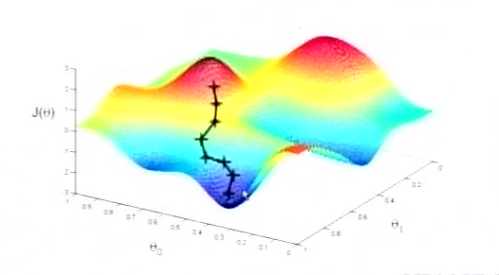
\includegraphics[scale=1.6]{grad1.png}
		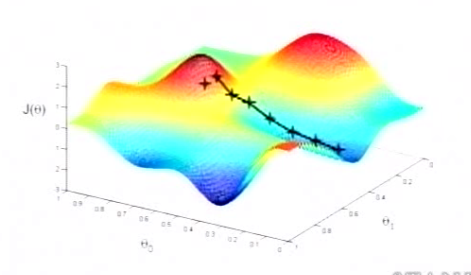
\includegraphics[scale=1.6]{grad2.png}
	\end{center}
}

\paragraph{Choix de $\alpha$}
Il est important de bien choisir $\alpha$, car si sa valeur est trop élevé il est possible que $J(\theta)$ croisse. Une valeur faible de $\alpha$ est donc préférable mais il faut savoir que plus sa valeur est faible, plus le temps de convergence sera long ...
\begin{center}
	\begin{tikzpicture}[thick, >={latex}, scale=0.9]
		\draw[domain=1.181978:6.956124, smooth, variable=\x, blue] 
			plot ({\x}, {0.5 * (\x - 4)^2});
		\draw[->, greenTikz]
			(2.000000, 2.000000) -- node[right] {\footnotesize petit $\alpha$} (3.500000, 0.125000);
		\draw[->, red]
			(2.000000, 2.000000) -- node[below] {\footnotesize grand $\alpha$} (6.160000, 2.332800);
		\draw[->, greenTikz] (3.500000, 0.125000) -- (3.875000, 0.007812);
		\draw[->, red] (6.160000, 2.332800) -- (1.667200, 2.720978);
		\draw[->, greenTikz] (3.875000, 0.007812) -- (3.968750, 0.000488);
		\draw[->, red] (1.667200, 2.720978) -- (6.519424, 3.173749);
		\draw[fill] (2, 2) circle (0.1);
	\end{tikzpicture}
\end{center}

\paragraph{Pour}
\begin{itemize}
	\item Peu de mises à jour sont nécessaires car le gradient est stable.
	\item La séparation en somme de la mise à jour permet d'utiliser des algorithmes parallèles
\end{itemize}
\paragraph{Contre}
\begin{itemize}
	\item La stabilité du gradient peu conduire prématurément vers un minimum local pas très optimal.
	\item La mise à jour peut prendre beaucoup de temps pour de grandes bases de données.
\end{itemize}

\subsubs{Descente de gradient stochastique}

Si la base de donnée est grande, disons 1 million d'exemples alors à chaque itération de le descente de gradient par batchs, on doit réaliser une somme d'erreurs sur un million d'exemples. Pour plus de rapidité il nous faut donc penser à un autre algorithme où l'on fait des mises à jour de $\theta$ plus régulièrement :

\begin{center}
	\begin{algorithm}[H]
		Initialisation de $\theta$\;
		\Repeat{convergence de $J(\theta)$}{
			\For{$j=1$ à $m$}{
				$\forall i, \; \theta_i \gets \theta_i - \alpha \left( h_\theta(x^{(j)}) - y^{(j)} \right) x_i^{(j)} $
			}
		}
		\caption{Descente de gradient stochastique}
	\end{algorithm}
\end{center}

\paragraph{Pour}
\begin{itemize}
	\item La fréquence élevé des mises à jour qui peut donner un apprentissage plus rapide.
	\item Ces mise à jours un peu "chaotiques" et instables peuvent empêcher de converger vers des minimas locaux.
	\item Cet algorithme permet aussi d'avoir un acquisition de données en ligne.
\end{itemize}
\paragraph{Contre}
L'algorithme ne converge pas vers le minimum globale mais il a tendance à rester autour.

\paragraph{Descente de gradient par mini-batchs}
Pour gagner en robustesse et garder l'efficacité de la descente stochastique, on peut séparer l'ensemble d'entraînement en de petits sous-ensembles (des petits batchs). Puis on reprend la descente stochastique mais au lieu de mettre à jour $\theta$ en s'appuyant sur un seul exemple à la fois, on le met à jour en fonction de l'erreur sur un mini-batch.

\subs{Solution de forme fermée}

On pose les vecteurs et matrices suivantes :
$$ x^{(j)} = \begin{pmatrix} x_0^{(j)} \\ \vdots \\ x_n^{(j)} \end{pmatrix} \qquad
X = \begin{pmatrix} {x^{(1)}}^\trans \\ \vdots \\ {x^{(m)}}^\trans \end{pmatrix} \qquad 
\theta = \begin{pmatrix} \theta_0 \\ \vdots \\ \theta_n \end{pmatrix} \qquad
y = \begin{pmatrix} y^{(1)} \\ \vdots \\ y^{(m)} \end{pmatrix} $$
Cela nous permet de réécrire $J(\theta)$.
$$ J(\theta) = \dfrac{1}{2m} (X\theta - y)^\trans (X\theta - y) $$
En un minimum de $J$, le gradient est nul. On cherche donc à résoudre :
$$ \nabla_\theta \dfrac{1}{2} (X\theta - y)^\trans (X\theta - y) = 0 $$
\newpage

$$ \begin{array}{lll}
\nabla_\theta \dfrac{1}{2} (X\theta - y)^\trans (X\theta - y)
& = & \dfrac{1}{2} \nabla_\theta \left( \theta^\trans X^\trans X \theta - \theta^\trans X^\trans y - y^\trans X \theta + y^\trans y \right) \\ \\
& = & \dfrac{1}{2} \left[ \nabla_\theta \left(\theta^\trans X^\trans X \theta \right) - 2 \nabla_\theta \left( y^\trans X \theta \right) \right] \\ \\
& = & X^\trans X \theta - X^\trans y
\end{array} $$

\PROP[ (Solution de forme fermée)]{
	Ainsi, si $X^\trans X$ est inversible, l'expression de $\theta$ suivante est optimale :
	\vspace{-1mm}
	$$\theta = (X^\trans X)^{-1} X^\trans y$$
	En revanche si $X^\trans X$ n'est pas inversible, il est possible que des features soient redondants. Appliqué l'algorithme PCA peut alors être une solution.
}

\subs{Régression polynomiale}

Dans le cas d'une régression polynomiale, on $h_\theta(x) = \theta_0 + \theta_1 x + \theta_2 x^2 + ... + \theta_n x^n$. La fonction est toujours linéaire selon $\theta$. L'idée est alors de se placer en dimension $n+1$, en posant $x_i = x^i$.

\sect{Interprétation probabiliste de la régression}

On peut se poser la question : Pourquoi les moindres carrées ? Pourquoi ne pas minimiser la valeur absolue ou encore la puissance 4 ?

Supposons que l'erreur sur $y^{(i)}$ suit une loi gaussienne. Ceci est justifié par le théorème centrale limite. On a donc :
$$ y^{(i)} = \theta^\trans x^{(i)} + \epsilon^{(i)} $$
Où $\epsilon^{(i)} \sim \mathcal{N}(0, \sigma)$. \\
On va ensuite chercher à maximiser la vraisemblance de $y$.

\DEF{
	Soit $X_1, ..., X_m$ des variables aléatoires i.i.d de densité $f(x|\theta)$ où $\theta$ est un paramètre de la loi. Pour un échantillon $X_1 = x_1, ..., X_n = x_n$ donné, la \textbf{vraisemblance} est : \vspace{-3mm}
	$$ L(\theta) = f(x_1, ..., x_n) = \prod_{i=1}^m f(x_i|\theta) $$
	\vspace{-7mm}
}

On a donc dans notre cas :
$$ L(\theta) = \Pp(y | X, \theta) = \prod_{i=1}^m \Pp(y^{(i)} | x^{(i)}, \theta) = \prod_{i=1}^m \dfrac{1}{\sqrt{2 \pi} \sigma} \exp \left( - \dfrac{(y^{(i)} - \theta^\trans x^{(i)})^2}{2 \sigma^2} \right) $$
Une bonne manière d'étudier la vraisemblance est de la passer au logarithme car elle est souvent log-concave. La log-vraisemblance est notée $l(\theta) = \ln L(\theta)$. Voici alors ce qu'on obtient si on simplifie l'expression de la log-vraisemblance :

$$ \begin{array}{lll}
	l(\theta)
	& = & \displaystyle \sum_{i = 1}^m \ln \left( \dfrac{1}{\sqrt{2 \pi} \sigma} \exp \left( - \dfrac{(y^{(i)} - \theta^\trans x^{(i)})^2}{2 \sigma^2} \right) \right) \\
	& = & \displaystyle \sum_{i = 1}^m \ln \dfrac{1}{\sqrt{2 \pi} \sigma} + \sum_{i = 1}^m \left( - \dfrac{(y^{(i)} - \theta^\trans x^{(i)})^2}{2 \sigma^2} \right) \\
	& = & \displaystyle m \ln \dfrac{1}{\sqrt{2 \pi} \sigma} - \sum_{i = 1}^m \dfrac{(y^{(i)} - \theta^\trans x^{(i)})^2}{2 \sigma^2}
\end{array} $$
Ainsi maximiser $l(\theta)$ revient à minimiser $\displaystyle J(\theta) = \sum_{i = 1}^m \dfrac{(y^{(i)} - \theta^\trans x^{(i)})^2}{2}$ \\
Donc lorsque l'on utilise l'algorithme des moindres carrées, on maximise simplement la vraisemblance en assumant que les erreurs sur les $y^{(i)}$ sont i.i.d selon une loi normale.

\sect{Régression régularisée}

Comme on l'a vu à la fin du chapitre précédent, il y a des risques d'overfitting. Une solution est la régularisation. On parle de régularisation \textbf{ridge} pour la norme $l_2$ et de régularisation \textbf{LASSO} pour la norme $l_1$.

\begin{center}
	\begin{tikzpicture}[thick, >={latex}]
	\draw[domain=0:360, smooth, variable=\t, very thick, fill=greenTikz, fill opacity=0.6]
	plot ({1.800000 + 3.035357 * cos(\t) + 0.443197 * sin(\t)}, {1.700000 + -1.107992 * cos(\t) + 1.214143 * sin(\t)});
	\draw[domain=0:360, smooth, variable=\t, very thick] 
	plot ({1.800000 + 0.758839 * cos(\t) + 0.110799 * sin(\t)}, {1.700000 + -0.276998 * cos(\t) + 0.303536 * sin(\t)});
	\draw[domain=0:360, smooth, variable=\t, very thick] 
	plot ({1.800000 + 1.517678 * cos(\t) + 0.221598 * sin(\t)}, {1.700000 + -0.553996 * cos(\t) + 0.607071 * sin(\t)});
	\draw[domain=0:360, smooth, variable=\t, very thick] 
	plot ({1.800000 + 2.276518 * cos(\t) + 0.332398 * sin(\t)}, {1.700000 + -0.830994 * cos(\t) + 0.910607 * sin(\t)});
	
	\draw[domain=0:360, smooth, variable=\t, very thick, fill=greenTikz, fill opacity=0.6]
	plot ({10.800000 + 3.289353 * cos(\t) + 0.480283 * sin(\t)}, {1.700000 + -1.200708 * cos(\t) + 1.315741 * sin(\t)});
	\draw[domain=0:360, smooth, variable=\t, very thick] 
	plot ({10.800000 + 0.822338 * cos(\t) + 0.120071 * sin(\t)}, {1.700000 + -0.300177 * cos(\t) + 0.328935 * sin(\t)});
	\draw[domain=0:360, smooth, variable=\t, very thick] 
	plot ({10.800000 + 1.644677 * cos(\t) + 0.240142 * sin(\t)}, {1.700000 + -0.600354 * cos(\t) + 0.657871 * sin(\t)});
	\draw[domain=0:360, smooth, variable=\t, very thick] 
	plot ({10.800000 + 2.467015 * cos(\t) + 0.360212 * sin(\t)}, {1.700000 + -0.900531 * cos(\t) + 0.986806 * sin(\t)});
	
	\draw[->] (0, -1.5) -- (0, 3.8);
	\draw[->] (-2, 0) -- (5, 0);
	\draw[->] (9, -1.5) -- (9, 3.8);
	\draw[->] (7, 0) -- (14, 0);
	\draw[very thick, fill=purple] (0, 0) circle (1);
	\draw[very thick, fill=purple] (9, 1) -- (8, 0) -- (9, -1) -- (10, 0) -- cycle;
	\fill[redLight] (9, 1) circle (0.16);
	\fill[redLight] (0.342898, 0.939373) circle (0.16);
	\node[red] at (4, 3.5) {Ridge};
	\node[red] at (13, 3.5) {LASSO};
	\end{tikzpicture}
\end{center}

\PROP[ (Forme fermée pour Ridge)]{
	Pour le régression ridge, la solution de forme fermée est la suivante :
	$$\theta = (X^\trans X + \lambda I_{n+1})^{-1} X^\trans y $$
	\vspace{-8mm}
}

\PROP[ (Stabilité uniforme pour Ridge)]{
	Avec la régression ridge, on obtient la borne de généralisation suivante :
	$$ \trisk(h_\theta) \leqslant \erisk(h_\theta) + \dfrac{4 B^2}{\lambda m} + \left( \dfrac{8 B^2}{\lambda} + 2B \right) \sqrt{\dfrac{\ln 1/\delta}{2m}} $$
	Où $\Y$ est bornée et $\Y = [0, B]$.
}

En revanche pour la régularisation LASSO, on ne dispose pas de résultats précis, mais on sait que l'utilisation de cette régularisation conduit à une diminution du nombre de paramètres non nuls. Ainsi LASSO permet d'avoir le vecteur $\bm{\theta}$ \textbf{creux}.

\sect{Machine à vecteur de support (SVR)}

Jusque là nous utilisé la méthode des moindres carrés. Il y a aussi la \textbf{perte $\bm{\epsilon}$-sensible} :
$$ \min_{\theta, \xi, \xi^*} \frac{1}{2} \| \theta \|_2^2 + C \sum_{i = 1}^m \left( \xi_i + \xi_i^* \right) $$
\vspace{-2mm}
$$ \text{s.t. } \left\{ \begin{array}{l}
	y^{(i)} - \theta^\trans x^{(i)} \leqslant \epsilon + \xi_i \\
	\theta^\trans x^{(i)} - y^{(i)} \leqslant \epsilon + \xi_i^* \\
	\xi_i, \xi_i^* \geqslant 0
\end{array} \right. $$

Le lagrangien de ce problème est alors le suivant :
$$ L(\theta, \xi, \xi^*, \alpha, \alpha^*, \beta, \beta^*) = \dfrac{1}{2} \| \theta \|^2 + C \mathbbm{1}_m^\trans \left( \xi + \xi^* \right) + \alpha^\trans \left( y - X \theta - \epsilon \mathbbm{1}_m - \xi \right) + {\alpha^*}^\trans \left( X \theta - y - \epsilon \mathbbm{1}_m - \xi \right) - \beta^\trans \xi - {\beta^*}^\trans \xi^*$$
On rappelle que la fonction objective du dual est :
$$ g(\alpha, \alpha^*, \beta, \beta^*) = \inf_{\theta, \xi, \xi^*} L(\theta, \xi, \xi^*, \alpha, \alpha^*, \beta, \beta^*) $$
On cherche maintenant ce que vaut $\theta$ dans l'expression de $g$.
$$ \dfrac{\partial L}{\partial \theta} = \theta - X^\trans \alpha + X^\trans \alpha^* $$
$$ \dfrac{\partial L}{\partial \xi} = C \mathbbm{1}_m - \alpha - \alpha^* - \beta \qquad \qquad
\dfrac{\partial L}{\partial \xi^*} = C \mathbbm{1}_m - \alpha - \alpha^* - \beta^* $$
D'où $\theta = X^\trans (\alpha - \alpha*)$ et $\beta = \beta^* = C \mathbbm{1} - (\alpha + \alpha^*)$. On obtient alors :
$$ g(\alpha, \alpha^*) = -\dfrac{1}{2} (\alpha - \alpha^*)^\trans X X^\trans (\alpha - \alpha^*) + (\alpha - \alpha^*)^\trans y - \epsilon (\alpha + \alpha^*)^\trans \mathbbm{1}_m $$
Et on a la condition $\alpha + \alpha^* \leqslant C \mathbbm{1}_m$ car $\beta$ et $\beta^*$ sont positifs. \\ Soit alors $(\alpha, \alpha^*)$ une solution. Supposons $\alpha \geqslant \alpha^*$. On pose $\nu = \alpha - \alpha^*$. On a alors $\nu \leqslant \alpha + \alpha^*$ et $\nu - 0 = \alpha - \alpha^*$. Donc $(\nu, 0)$ est aussi une solution, et $g(\nu, 0) \geqslant g(\alpha, \alpha^*)$. \\
On obtient finalement le problème dual suivant :
\begin{center}
	\fbox{$ \displaystyle \min_{|\nu_i| \leqslant C} \dfrac{1}{2} \left\| X^\trans \nu \right\|_2^2 - \nu^\trans y + \epsilon \| \nu \|_1 $}
\end{center}
Dans ce cas, on a $\theta = X^\trans \nu$, et $h_\nu(x) = \theta^\trans x = \nu^\trans X x$.

\paragraph{Astuce du noyau}
Dans le cas non, linéaire il existe une astuce du noyau. Il est bon de le savoir mais je ne vais pas en parler ici.

\sect{De la régression à la classification}

\subs{Régression logistique}

Jusqu'à maintenant, nous avons considéré $y \in \R$. On se place désormais dans le cas où $y \in \{0, 1\}$. Par exemple $y = 1$ lorsque le patient a une maladie et $y = 0$ sinon. Dans ce cas c'est généralement une  mauvaise idée d'utiliser un régression linéaire.

\begin{center}
	\begin{tikzpicture}[scale=2, thick, >={latex}]
		\draw[->] (-0.2, 0) -- (2.3, 0);
		\draw[->] (0, -0.2) -- (0, 1.3);
		\draw[fill=blue] (0.2, 0) circle(0.04);
		\draw[fill=blue] (0.3, 0) circle(0.04);
		\draw[fill=blue] (0.4, 0) circle(0.04);
		\draw[fill=blue] (0.5, 0) circle(0.04);
		\draw[fill=blue] (0.6, 1) circle(0.04);
		\draw[fill=blue] (0.7, 1) circle(0.04);
		\draw[fill=blue] (0.8, 1) circle(0.04);
		\draw[fill=blue] (0.9, 1) circle(0.04);
		\draw[fill=blue] (2, 1) circle(0.04);
		\draw[domain=0:1.8, smooth, variable=\x, red] plot ({\x}, {0.107+0.631*\x});
	\end{tikzpicture}
\end{center}

On utilise alors la régression logistique.

\DEF{
	La fonction \textbf{sigmoïde (logistique)} est définie par :
	$$ sig(z) = \dfrac{1}{1 + e^{-z}} $$
	\vspace{-3mm}
	Et sa fonction réciproque, la fonction \textbf{logit} est définie par :
	$$ logit(p) = \ln \left( \dfrac{p}{1-p} \right) $$
	\vspace{-6mm}
}

Cette fonction nous permet de définir le nouveau modèle :
\begin{center}
	\boldmath \fbox{$ \displaystyle h_\theta(x) = g \left( \theta^\trans x \right) = \dfrac{1}{1 + e^{-\theta^\trans x}} $}
\end{center}

\begin{center}
	\begin{tikzpicture}[scale=2, thick, >={latex}]
	\draw[->] (-0.2, 0) -- (2.3, 0);
	\draw[->] (0, -0.2) -- (0, 1.3);
	\draw[fill=blue] (0.2, 0) circle(0.04);
	\draw[fill=blue] (0.3, 0) circle(0.04);
	\draw[fill=blue] (0.4, 0) circle(0.04);
	\draw[fill=blue] (0.5, 0) circle(0.04);
	\draw[fill=blue] (0.6, 1) circle(0.04);
	\draw[fill=blue] (0.7, 1) circle(0.04);
	\draw[fill=blue] (0.8, 1) circle(0.04);
	\draw[fill=blue] (0.9, 1) circle(0.04);
	\draw[fill=blue] (2, 1) circle(0.04);
	\draw[domain=0.3:2, smooth, variable=\x, greenTikz, ultra thick] plot ({\x}, {1 / (1 + exp(-30.1*\x+16.55))});
	\draw[ultra thick, greenTikz] (0, 0) -- (0.3, 0);
	\end{tikzpicture}
\end{center}

Ainsi si $\theta^\trans > 0$ alors $h_\theta(x) > \frac{1}{2}$ et on pose $\hat{y} = 1$ sinon on pose $\hat{y} = 0$. On peut voir $h_\theta(x)$ comme une probabilité tel que $\Pp(y = 1|x, \theta) = h_\theta(x)$. \\
La méthode des moindres carrées est adaptée pour la régression mais pour la classification on préfère maximiser la vraisemblance puisque $h_\theta$ représente une probabilité.
$$ \Pp(y = 1 | x, \theta) = h_\theta(x) \qquad \text{et} \qquad \Pp(y = 0 | x, \theta) = 1 - h_\theta(x) $$
Cela nous donne :
$$ \Pp(y | x, \theta) = h_\theta(x)^y \left( 1 - h_\theta(x) \right)^{1-y} $$
On en déduit ensuite la vraisemblance :
$$ L(\theta) = \prod_{i=1}^m \Pp(y^{(i)} | x^{(i)}, \theta) = \prod_{i=1}^m h_\theta(x^{(i)})^{y^{(i)}} \left( 1 - h_\theta(x^{(i)}) \right)^{1-y^{(i)}}$$
Comme dit précédemment, il est plus facile de maximiser la log-vraisemblance :
$$ l(\theta) = \sum_{i = 1}^m y^{(i)} \ln \left( h_\theta(x^{(i)}) \right) + (1 - y^{(i)}) \ln \left( 1 - h_\theta(x^{(i)}) \right) $$
De la même manière qu'en régression linéaire, on va faire une ascension de gradient (et non plus une descente car ici on cherche à maximiser une vraisemblance et non à minimiser une distance).
$$ \theta_j \gets \theta_j + \alpha \dfrac{\partial}{\partial \theta_j} l(\theta) $$
Il nous faut alors calculer le gradient :
$$ \dfrac{\partial}{\partial \theta_j} l(\theta) = \sum_{i = 1}^m \left( y^{(i)} - h_\theta(x^{(i)}) \right) x_j^{(i)} $$
On obtient finalement :
\begin{center}
	\boldmath \fbox{$ \displaystyle \theta_j \gets \theta_j + \alpha \sum_{i = 1}^m \left( y^{(i)} - h_\theta(x^{(i)}) \right) x_j^{(i)} $}
\end{center}
On obtient exactement la même solution que pour la méthode des moindres carrés.

\paragraph{C'est un modèle linéaire} Nous avons dit que $\hat{y}$ vaut 1 si et seulement si $h_\theta(x)$ est plus grand que $\frac{1}{2}$. Or $h_\theta(x) > \frac{1}{2} \Leftrightarrow \theta^\trans x > 0$. Derrière cette régression logistique il y a finalement un modèle linéaire où l'hyperplan $\theta^\trans x = 0$ sépare l'espace en deux.

\begin{center}
	\begin{tikzpicture}[thick, scale=0.8]
		\draw[fill, red] (0, 1) circle (0.1);
		\draw[fill, red] (1, 2) circle (0.1);
		\draw[fill, red] (2, 2) circle (0.1);
		\draw[fill, blue] (5, 4) circle (0.1);
		\draw[fill, blue] (3, 4) circle (0.1);
		\draw[fill, blue] (2, 5) circle (0.1);
		\draw[fill, blue] (2, 4) circle (0.1);
		\draw[greenTikz, ultra thick] (-0.5, 3.13) -- (5.5, 2.54)
			node[right, black] {$\theta^\trans x = 0$};
		\draw[gray!40] (-0.5, 0.5) rectangle (5.5, 5.5);
	\end{tikzpicture}
\end{center}

\subs{Méthode de Newton}

Il existe une méthode plus rapide que l'ascension de gradient. Cette méthode est la méthode de Newton qui consiste à trouver le zéro du gradient de la log-vraisemblance.

\begin{center}
	\begin{tikzpicture}[xscale=2.8, yscale=1.7, >={latex}]
		\draw[->] (-0.1, 0) -- (2.2, 0);
		\draw[->] (0, -0.3) -- (0, 2.1);
		\draw[domain=0.1:2, smooth, variable=\x, blue, thick]
			plot ({\x}, {-0.686 + \x * (4.72 + \x * (-7.3 + \x * (4.53 + \x * -0.858)))});
		\coordinate (A) at (1.800000, 0.000000);
		\coordinate (B) at (1.800000, 1.559280);
		\coordinate (C) at (1.164304, 0.000000);
		\coordinate (D) at (1.164304, 0.479580);
		\coordinate (E) at (0.498177, 0.000000);
		\coordinate (F) at (0.498177, 0.358360);
		\draw[red, thick] (A) -- node[right] {\footnotesize $f(\theta^0)$} (B)
			-- (C) -- node[below] {\footnotesize $\Delta$} (A);
		\draw[dotted, greenTikz, thick] (C) -- (D) -- (E) -- (F);
		\draw[greenTikz] (A) node {$\bullet$} node[below, black] {\small $\theta^0$};
		\draw[greenTikz] (B) node {$\bullet$};
		\draw[greenTikz] (C) node {$\bullet$} node[below, black] {\small $\theta^1$};
		\draw[greenTikz] (D) node {$\bullet$};
		\draw[greenTikz] (E) node {$\bullet$} node[below, black] {\small $\theta^2$};
		\draw[greenTikz] (F) node {$\bullet$};
		\draw[red] (0.2, 0) node {$\bullet$};
	\end{tikzpicture}
\end{center}

La relation de récurrence pour faire converger $\theta$ vers le zéro d'une fonction $f$ est alors :
$$ \theta^{t+1} = \theta^t - \Delta = \theta^t - \dfrac{f(\theta^t)}{f'(\theta^t)} $$
Dans notre cas la fonction $f$ est $l'$, le gradient de la log-vraisemblance. On obtient :
\begin{center}
	\boldmath \fbox{$ \displaystyle \theta^{t+1} = \theta^t - H^{-1} \nabla_\theta l(\theta^t) $}
\end{center}
Où $H$ est la matrice hessienne $ \displaystyle H = \begin{pmatrix}
	\dfrac{\partial^2 l}{\partial \theta_0^2} & \dots & \dfrac{\partial^2 l}{\partial \theta_0 \theta_n} \\
	\vdots & \ddots & \vdots \\
	\dfrac{\partial^2 l}{\partial \theta_n \theta_0} & \dots & \dfrac{\partial^2 l}{\partial \theta_n^2}
\end{pmatrix} $ et $\nabla_\theta l$ est le gradient de $l$.

\paragraph{Avantage} Pour un nombre raisonnable de features, et d'exemples d'entraînement, la méthode de Newton converge bien plus rapidement.
\paragraph{Désavantage} A chaque itération, on doit inverser la matrice hessienne de taille $(n+1) \times (n+1)$. Ainsi si $n$ est grand alors cette inversion est très coûteuse.
	
\end{document}